\documentclass{patmorin}
\usepackage{amsthm,amsmath,graphicx,stmaryrd}
\usepackage{pat}
\usepackage{wrapfig,url}

\DeclareMathOperator{\erf}{erf}
\DeclareMathOperator{\area}{area}
\newcommand{\eps}{\varepsilon}

\title{\MakeUppercase{Open Problems for Bellairs Workshop on Geometry and Graph}}
\author{BWGG 2013 Participants}
\newcommand{\poser}[1]{\noindent{\textit{#1}}}

\begin{document}
\begin{titlepage}
\maketitle

\begin{abstract}
  This document contains open problems provided by the participants of
  the Bellairs Workshop on Geometry and Graphs, March 10--15, 2013.
\end{abstract}
\end{titlepage}

\tableofcontents
\newpage

%===================================================================
\section{Graph Theory}
%===================================================================

%=============
\subsection{Average degree needed to guarantee a minor of size $k$}

\poser{Bruce Reed}

There exists a function, $f(k)$, such that any graph, $G$, with average
degree at least $f(k)$ contains every graph, $H$, with $k$ vertices as
a minor.

\begin{op}
  What is the function $f(k)$?
\end{op}

Average degree $O(k\log k)$ suffices for any $H$. Average degree $k-2$
or less is not enough.  The case of trees and other low density graphs
is of particular interest.

\section{Geometry}

%=============
\subsection{Hadwiger-Debrunner problems}

\poser{Bill Steiger}                 

\begin{op}
  Given a family $\mathcal{F}$ of convex bodies in $\R^2$ among which,
  for every four of them, some three must have a point in common, the
  problem is to determine $k$, the \emph{smallest} number of points
  in $\R^2$ that meet every set in $\mathcal{F}$ . $k$ is the piercing
  number of $\mathcal{F}$ .
\end{op}

This is an example of Hadwiger-Debrunner $(p,q,d)$ which asks the same
question for convex bodies in $\R^d$ for which, among every $p\ge q$
of them, some $q > d$ of them have non-empty intersection. Helly’s
Theorem is for $q = p = d + 1$, when the sets are pierced by $k = 1$
point; the $(4,3,2)$ problem is the first non-trivial case beyond Helly.
Alon and Kleitman (1992) had proved the conjecture of Hadwiger and
Debrunner---that $k$ is finite, and independent of the number of sets
in $\mathcal{F}$. When applied to the case $p = 4$, $q = 3$, $d = 2$,
their arguments for the general case showed that about 200 points would
always be sufficient to pierce $\mathcal{F}$.

Then in 2001, Kleitman, Gyarfas, and Toth proved that $k\le 13$, and
a simple construction with 6 triangles shows that $k\ge 3$. They offer
money for narrowing this gap, $\$5x$ for reducing the upper bound by $x$
and $\$10y$ for increasing the lower bound by $y$.  I think there are
better bounds for special families of convex sets, e.g. unit discs. I
think this is a hard problem, but who knows?


%=============
\subsection{Shortest paths among transparent obstructions}

\poser{Henk Meijer}                 

I am not sure what to call this. I started on this problem two years ago
with the following question: Suppose we have a helicopter at a point $A$,
and it needs to find the shortest flight path to point $B$. The speed of
the helicopter increases with height.  The shortest path of the helicopter
is then something that looks like a circular arc from $A$ to $B$.

One of my colleagues pointed out that this type  of problem  is exactly
what seismologists have been studying:  a seismic wave increases it
speed the deeper it gets.  The shortest/fastest path problem between
two points was for example already studied by someone named Gutenberg,
who lived in the first half of the 20th century.  I have been reading
about him in a standard textbook on seismology entitled "quantitative
seismology" by Aki and Richards, 1980.

I don't think we should try compete with the seismologists.  However it
raised the following question: Suppose we have a partition of the plane
into regions and two points $A$ and $B$.  Each region $p$ is associated
with a speed $s_p$.  Problem: compute the fastest path from $A$ to $B$,
such that the speed with which we can travel in region $p$ is $s_p$.

In the summer of 2011 a student of mine, Jelte Mense, started with this
problem. He constructed a shortest path map in case of a partition that
consisted of a single unit square in the plane, and a fixed point $A$.
The shortest path map divides the plane in combinatorially equal regions,
i.e. for each point in a region, the shortest path from $A$ intersects
the same features of the unit square.

There is virtually nothing know about this problem. Some possible 
questions:  

\begin{op}
  what is the complexity of finding the fastest path
\end{op}

\begin{op}
  does the shortest path map consists of quadratic shapes (hyperbolas,
  straight lines, $\ldots$ )
\end{op}

\begin{op}
  what is the combinatorial complexity of the shortest path map
\end{op}

\begin{op}
  how can we compute the fastest path from a point $A$ to a point $B$
\end{op}


The only thing that I know comes from physics. We know that light that
travels from $A$ to $B$ finds the shortest path from $A$ to $B$. If it
moves from a material in which it travels with speed $s_1$ to a material
in which it travels with speed $s_2$, the light is refracted. You might
recall the refraction formula
\[ 
   \frac{\sin \Theta_1}{\sin \Theta_2} ~=~ \frac{s_1}{s_2}
\]
where $\Theta_1$ and $\Theta_2$ are the angles between light rays and
surface normals.

Related work (from Pat):  Mitchell and Papadimitriou \cite{mp91} study the
problem of computing shortest paths in weighted domains.  They give
$(1+\epsilon)$-approximations whose running time is $O(n^8L)$ where $L$
represents the bit complexity of the problem instance.  See also Mata
and Mitchell \cite{mm97}, and Aleksandrov \etal\ \cite{ams05}.

%================
\subsection{External-memory LIDAR range searching}

\poser{Rolf Fagerberg}

At CCCG 2012, MacGillivray and Nickerson studied a 2D range search
problem motivated by aggregating overlapping LIDAR surveys of
landscapes. The data contains m point sets with polygonal boundaries
(i.e., $m$ LIDAR surveys), and a query is specified by an axis-aligned
query rectangle $R$ and a subset of the $m$ point sets. The query answer
should be the points stored in the selected point sets and lying inside
$R$---but where point sets (i.e., their polygonal boundaries) overlap,
only the points of the latest (highest indexed) point set should be
reported.

The paper gives an external memory structure with linear space and query
time $\sqrt{mN/B} + m^2 + K/B$. Here, $N$ is the total number of points, $K$ is
the output size, and $B$ is the block size.

\begin{op}
  The goal would be to improve the preceding result, e.g. by a better
  running time or a more general query type.
\end{op}


%=============
\subsection{Covering points with  disks}  

\poser{Greg Aloupis}


\begin{op}
  How many points must be placed in the plane so that no collection of
  disjoint unit disks can cover them?
\end{op}


This is a problem that has been around since at least 2008.
The upper bound has slowly trickled down from around 60 to 45; see
\url{http://2012.cccg.ca/papers/paper13.pdf}.

For all upper bounds of 50 or greater,  constructions have  involved
triangular grids, generated by the equilateral triangle that has
three points on the largest  circle that fits inside the gap created
by three mutually tangent unit disjoint disks.  Finally, a much more
sparse-looking set of 45 points was given, but the proof relied on an
exhaustive computer search.

The lower bound is 13, meaning any set of 12 points can be covered.
It is given in the link above, and is a refinement of a lower bound of
11 by  Inaba, who used the probabilistic method. See the appendix of:
\url{http://2011.cccg.ca/PDFschedule/papers/paper5.pdf}

\begin{op}
  What is the best bound for point sets embedded on grids?
  (Just asking for grid points is vague.  Suppose that the minimum distance
  between points in a grid is $d$, and let $G$ be the graph obtained
  by adding an edge between every pair of points with distance $d$.
  I'd accept any point set for which $G$ is connected.  This applies to
  the upper bounds of 50 and up; in fact they are very compact.  I  think
  there is little room for improvement).
\end{op}

\begin{op}
  For what value of $d$ does the following hold: Given any planar point
  set $S$, if the minimum distance between any pair of points is $d$,
  then $S$ can be covered by disjoint unit disks.
\end{op}

Clearly if $d$ is  the side length of the equilateral triangle mentioned
previously, then there are point sets that cannot be covered.   This value
is equal to $2-2\cos\frac{\pi}{6} = 2{-}\sqrt{3}$.  On the other hand, if
$d$ is $1$, then placing disks centered at every point will cover the set.

%==================
\subsection{Inverse range searching on bicoloured points}

\poser{Stephane Durocher}

This problem was previously discussed with members of my research group:
Robert Fraser, Saeed Mehrabi, Debajyoti Mondal, Jason Morrison, 
and Matthew Skala.

\begin{op}
  Given a set $P$ of $n$ points in the plane, each of which is coloured
  blue or red, and a pair of positive integers $b$ and $r$, Find an
  axis-parallel rectangle that contains exactly $b$ blue points and $r$
  red points of $P$.
\end{op}

The two-dimensional problem is motivated by the following one-dimensional
version which has applications in bioinformatics.  Given binary strings
$A$ and $B$ with respective lengths $n$ and $m < n$ as input, does $A$
contain a permutation of $B$ as a (continuous) substring?  Clearly this
problem can be solved in $O(n)$ time in a single pass over $A$.

We believe the problem has not been examined in a geometric setting
in two or more dimensions.  In two dimensions, $\Theta(n^4)$ distinct
subsets of $P$ can be enclosed by respective axis-parallel rectangles
due to the fact that the point of $P$ closest to each of the four edges
of the rectangle can be selected in $\Theta(n)$ ways.

A simple brute force approach is to build respective orthogonal range
counting data structures for the blue and red points.  Counting blue and
red points in each possible rectangle then requires $O(n^4 \log n)$ time.
The time can be improved to $O(n^3)$ by observing that for any pair
of horizontal lines, $\ell_1$ and $\ell_2$, and any fixed integer $b$,
at most $O(n)$ rectangles can contain exactly $b$ blue points of $P$,
where the rectangles top and bottom edges are determined by $\ell_1$
and $\ell_2$.  For each of the $\Theta(n^2)$ pairs of horizontal lines,
it suffices to enumerate the points in $P$ contained between $\ell_1$ and
$\ell_2$ ordered by $x$-coordinates, and to maintain indices corresponding
to the left and right vertical edges of the rectangles such that the
number of blue points between the indices remains exactly $b$.  If at
any time the number of red points between the indices is exactly $r$,
then return the rectangle determined by $\ell_1$, $\ell_2$, and the
left and right indices.  Furthermore, the points between $\ell_1$ and
$\ell_2$ need not be re-sorted each time $\ell_1$ or $\ell_2$ changes;
if the the horizontal lines are moved up or down one point at a time,
then the $x$-ordering of the points between the lines can be maintained
using a basic balanced search tree.

Can this problem be solved in $o(n^3)$ time?  Do Ham Sandwich type
results help?




\section{Geometric Graph Theory}

%=============
\subsection{Distinct embeddings of planar graphs}

\poser{Fabrizio Frati}

Given a planar graph, $G=(V,E)$, and a point set, $P$, a \emph{planar
straight-line embedding} of $G$ into $P$ is a mapping $V\to P$ such
that the resulting straight-line drawing of $G$ is planar.  Two planar
straight-line embeddings of $G$ into $P$ are distinct if the mapping
$V\to P$ is not the same.


\begin{op}
  What is the maximum (over $G$ and $P$) number of distinct straight-line
  planar embeddings of a maximal planar graph, $G$, into a point set, $P$?
\end{op}

The best known upper bound is roughly $30^n$ (which is the number of
triangulation of a point set \cite{s12}).  The best known
lower bound is $2^{n/3}$ (provided by the nested triangle graph and a
suitable point set).


%=============
\subsection{The cocktail party clinking problem}

\poser{David Wood}

\begin{wrapfigure}{r}{71mm}
\hfill
\includegraphics[width=70mm]{party}
\end{wrapfigure}
People are standing around at a cocktail party,  and the host calls a
toast. All the people want to clink glasses, but to avoid spillage, they
do not want their arms to cross while clinking. How many rounds of clinks
are sufficient for everyone to clink glasses? Naturally, we assume that
each person can clink with at most one other person in each round, no
three people are standing in a line, and everyone has long straight arms!

Put another way, for a set $P$ of $n$ points in general position in
the plane, let $f(P)$ be the minimum integer such that the edges of the
complete geometric graph on $P$ can be coloured with $f(P)$ colours, such
that each colour class is a non-crossing matching. That is, monochromatic
edges do not intersect (including at a common endpoint). Let $f(n)$ be
the maximum of $f(P)$ taken over every set $P$ of $n$ points in general
position in the plane.

\begin{op}
  What is $f(n)$? 
\end{op}

Araujo \emph{et al.}~\cite{Araujo} proved that
$f(n)\in\mathcal{O}(n^{3/2})$, but the best known lower bound is
$\Omega(n)$. So there is a huge gap in the bounds, and the problem is
ripe for attack. I conjecture that $f(n)\in\mathcal{O}(n)$. Surely,
$f(n)\in\mathcal{O}(n\text{ polylog } n)$ is true.

\begin{wrapfigure}{l}{61mm}

\includegraphics[width=6cm]{dinner}
\end{wrapfigure}

The related dinner party clinking problem is solved. Here, our point
set $P$ is in convex position, and $f(P)=n$. Why? Say Vida is sitting
between Jit and Pat. It takes at least $n-1$ rounds for Vida to clink
with the $n-1$ other people, and Vida does not clink in the round in
which Jit and Pat clink. So at least $n$ rounds are needed. For the upper
bound, number the people $1,2,\dots,n$ around the table. Then the $i$-th
person clinks with the $j$-th person in the $k$-th round if and only if
$i+j\equiv k\pmod{n}$.

\ % deliberately placed here to fix wrapfigure

%=============
\subsection{The sexy points problem}

\poser{David Wood}

\begin{wrapfigure}{r}{67mm}
\hfill
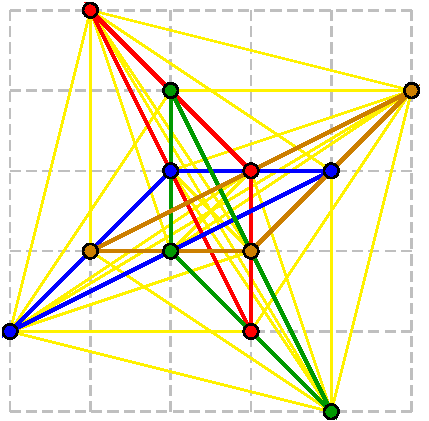
\includegraphics[width=67mm]{K3333}
\end{wrapfigure}
Given a set $P$ of points in the plane, two points $x,y\in P$
are \emph{visible} if no point in $P$ lies on the open line segment
$\overline{xy}$. A set of coloured points in the plane is \emph{sexy}
if two points are visible if and only if they have distinct colours. If
there are $k$ colours, then the point set is \emph{$k$-sexy}. The figure
shows an example of a 4-sexy set with 12 points.

\begin{op}
  Resolve the following conjecture: Every $k$-sexy set has at most $f(k)$
  points, for some function $f$.
\end{op}

For example, every 1-sexy  set has at most 1 point, every 2-sexy set
has at most 3 points, every 3-sexy set has at most 6 points \cite{Kara},
and every 4-sexy set has at most 12 points \cite{Aloupis}. With enough
case analysis, the methods developed in \cite{Aloupis} could probably
prove that $f(5)$ is finite, but this is not as interesting as the
general question.

The conjecture can be restated as follows:  for fixed $k$,  arbitrarily
large complete $k$-partite graphs are not visibility graphs. This a
special case of a number of deep and challenging conjectures about
visibility graphs \cite{Kara,Por}. So one would hope that the methods
developed for the solution of the above conjecture would be useful for
other problems.

%=====================
\subsection{Flip distance between triangulations with common subgraphs}

\poser{Jit Bose}

Given two distinct triangulations on the same set of $n$ points in the
plane, Hanke, Ottmann, and Schuierer showed how to convert one
triangulation into the other such that number of flips does not exceed
the number of intersections when you overlay the two triangulations.
In the worst case, this provides an upper bound of $(3n-6)^2$.

\begin{op}
  Let $T_1$ and $T_2$ be two triangulations of the same point set that
  have $k$ edges in common.  How many geometric flips are required to
  convert $T_1$ into $T_2$?  How does this bound depend on $k$?
\end{op}

For example, the Delaunay triangulation and the Greedy triangulation both
share the minimum spanning tree. Can they still be a quadratic number of
flips apart or is it possible to convert one to the other with $o(n^2)$
flips?


\subsection{Drawing simultaneous planar graphs}

\poser{Anna Lubiw}

Let $G_1$ and $G_2$ be planar graphs with a common subgraph $G$.
We say that $G_1$ and $G_2$ are \emph{simultaneously planar} if there
is a drawing of $G_1 \cup G_2$ where crossings may only occur between
edges of $G_1 - G$ and edges of $G_2 - G$ (i.e.~ between ``private''
edge of $G_1$ and private edges of $G_2$).  

\begin{op}
  Find a simultaneous planar drawing of $G_1$ and $G_2$ with few edge
  bends.
\end{op}

There are examples where bends are required in any simultaneous planar
drawing.

The case where $G$ is connected is particularly interesting because
in that case $G_1$ and $G_2$ are simultaneously planar iff they each
have a planar rotation system (an ordering of edges around each vertex)
such that common edges appear in the same order~\cite{Junger-Schulz}.

The best known result~\cite{Haeupler-13} is that if $G$ is connected
then there is a simultaneous planar drawing where edges of $G_1$ have
no bends and each  edge of $G_2$ has at most $n$ bends, where $n$ is
the number of vertices of $G$.  Furthermore, a private edge of $G_1$
crosses a private edge of $G_2$ at most once.  However, there is no nice
bound on vertex coordinates.

It is open to reduce the number of bends and/or to put the drawing on
a nice grid.

\subsection{Morphing planar graphs with minimum movement}

\poser{Anna Lubiw}

\begin{op}
  Given two planar drawings of the same planar graph find a \emph{morph}
  (a continuous planarity-preserving transformation) between them that
  minimizes the maximum distance that any vertex or any point on an
  edge travels.
\end{op}

This is  like asking for  the Fr\'echet distance between the two
drawings, with some continuity conditions.  It generalizes the
homotopic Fr\'echet distance between two planar curves in the presence
of obstacles~\cite{Chambers-10}.

A related problem is to morph between two graph drawings where the
motion of every vertex and every point on an edge is limited to some
maximum speed.  How much time does it take to morph from one drawing to
the other?  (There is work on Fr\'echet distance of curves with speed
limits~\cite{Maheshwari-11}, but this does not generalize that.)

There are basically three known methods for morphing planar graph
drawings:

\begin{enumerate}
\item a ``discrete'' method due to Cairns, recently made polynomial time~\cite{poly-morph}
\item a method that allows edges to bend~\cite{Lubiw-Petrick}
\item an implicitly defined morph by Floater and Gotsman~\cite{Floater-Gotsman}
\end{enumerate}

I don't know how any of these behaves in terms of the distance each
point travels.

%=========================
\subsection{Shortest paths in 3-d meshes}

\poser{Stefanie Wuhrer}

Many applications in geometry processing require the computation of
shortest geodesic paths on surfaces represented by triangle meshes. It
is often sufficient to use shortest paths on the graph induced by the
vertices and edges of the triangulation. That is, we are interested
in computing shortest paths on a graph $G$ with $n$ vertices and $m$
edges, where the weight of each edge is its Euclidean length. In our
case, the graph has the following properties: vertices are embedded in
$\mathbb{R}^3$, every face is a triangle, every edge has two adjacent
triangles, and the triangles incident on a vertex $p$ of $G$ can be
cyclically ordered around $p$. Hence, for surfaces of constant genus,
$m$ is $O(n)$.

To solve the single source shortest path (SSSP) problem on $G$,
Dijkstra's algorithm takes $O(m + n \log n)$ time, so $O(n \log n)$
time in our case. To solve the all pairs shortest path (APSP) problem,
we can run Dijkstra's algorithm starting from each source point, yielding
$O(n^2 \log n)$ time. While there are more efficient methods, the APSP
problem has a $\Omega(n^2)$ lower bound.

For large meshes, it is impractical to use algorithms that take
$\Omega(n^2)$ time. A commonly used approach to reduce the complexity
is to select $k$ sources, to solve the SSSP problem from these
sources, and to approximate the remaining distances. Several methods
that approximate APSP using distances from $k$ SSSP computations
proceed by finding an embedding of the vertices of $G$ in a Euclidean
space based on the computed distances and by approximating (unknown)
distances on $G$ using Euclidean distances in the embedding space, see
e.g.~\cite{giard_macq_09_unfold, BenAzouz_etal_07}. However, no bounds
on the error of such approximations is known.

Consider $p$ and $q$ on $G$, and let $d(p,q)$ denote the shortest distance
between $p$ and $q$ on $G$. After solving the SSSP problem for $k$ sources
$s_1,s_2,\ldots,s_k$, we can use the triangle inequality to find an upper
bound on $d(p,q)$ as $d^u(p,q) = \min_i(d(p,s_i)+d(q,s_i))$. A trivial
lower bound on $d(p,q)$ is the Euclidean distance between $p$ and $q$.

To the best of my knowledge, the following are open problems:

\begin{op}
Given a number, $k$, where should we place the $k$ sources used for SSSP,
such that $\max_{p,q} \frac{d^u(p,q)}{d(p,q)}$ is minimized?
\end{op}
(A commonly used technique in practice is to use Voronoi sampling to place the sources. Can this be shown to be an optimal choice?)

\begin{op}
Given a number $k$ of sources, can we find a placement
of the sources that allows us to derive a bound on $\max_{p,q}
\frac{d^u(p,q)}{d(p,q)}$?
\end{op}

%===============
\subsection{Non-crossing graphs on 3-d grids}

\poser{Vida Dujmovi\'c}

\begin{op}
  What is the maximum number of non-crossing graphs that can be
  drawn on the $2\times\sqrt{n}\times\sqrt{n}$ grid 
  \[ \{(x,y,z):
  x,y\in\{1,\ldots,\sqrt{n}\},\, z\in\{1,2\}\} \enspace ? \]
\end{op}

The answer to the equivalent problems in dimensions $d=2$ and $d\ge 4$
is known.  In 2 dimensions, the maximum number of non-crossing graphs
that can be drawn on any point set is $2^{O(n)}$ \cite{acns82} and 
$2^{\Omega(n)}$ graphs can be drawn on the $2\times n$ grid.
In 4 and higher dimensions, the maximum number of non-crossing graphs
that can be drawn on a $2\times n^{1/(d-1)}\times\cdots\times n^{1/(d-1)}$
grid with $n$ points $2^{\Theta(n\log n)}$ \cite{dms13}.

%===============
\subsection{Separating crossing angles from geometric thickness}

\poser{Pat Morin}

A geometric graph, $G$, is called \emph{$\alpha$-AC} if it can be drawn in
the plane so that any two edges that cross each other do so at an angle of
at least $\alpha$.  If $G$ is $\alpha$-AC then the edges of this drawing
can easily be colored with $\lceil\pi/\alpha\rceil$ colors so that no
two edges of the same color cross each other. Therefore any $\alpha$-AC
graph has \emph{geometric thickness} at most $\lceil\pi/\alpha\rceil$.

\begin{op}
  Prove or disprove:  There are graphs of geometric thickness $k$ that
  are not $\alpha$-AC for any $\alpha$ of the form $\pi/f(k)$.
\end{op}

%================
\subsection{Obstacle numbers}

\poser{Vida Dujmovi\'c}

An obstacle representation of a graph, $G=(V,E)$, is a set $V'$ of
points in the plane together with a set of opaque connected obstacles
such that $G$ is isomorphic the visibility graph on $V'$ determined
by the obstacles. That is, an edge $uw\in E$  if and only if the
line segment joining the corresponding points, $u'$ and $w'$, in $V'$
does not intersect any obstacles. The \emph{obstacle number} of $G$ is
the minimum number of obstacles in an obstacle representation of $G$.

It is not hard to see that the obstacle number of $G$ is at most
$\binom{n}{2}-|E|$.  It is known that every outerplanar graph has obstacle
number 1 \cite{akl10}.

\begin{op}
  Is the obstacle number of a graph with $n$ vertices bounded above by
  a linear function of $n$?
\end{op}

Mukkamala, Pach, and Sari\"oz \cite{mps10} give examples of graphs with
obstacle number $\Omega(n/\log^2 n)$.

\begin{op}
  Determine upper and lower bounds on the obstacle number of some non-trivial classes of graphs.
\end{op}

Both references above also consider other variants, including convex
obstacles and polygonal obstacles with few sides.



\bibliographystyle{plainnat}
\begin{thebibliography}{1}

\newcommand{\doi}[1]{}

% Henk
\bibitem{mp91}
J.S.B. Mitchell and C.H. Papadimitriou, ``The Weighted Region Problem: Finding
Shortest Paths Through a Weighted Planar Subdivision'', Journal of the ACM, 38,
January 1991, pp.~18--73.

\bibitem{mm97}
C. Mata and J. Mitchell, ``A New Algorithm for Computing Shortest Paths in
Weighted Planar Subdivisions'', Proceedings of the 13th Annual ACM Symposium
on Computational Geometry, 1997, pp. 264-273.

\bibitem{ams05}
Lyudmil Aleksandrov, Anil Maheshwari, J\"org-R\"udiger Sack: Determining
approximate shortest paths on weighted polyhedral surfaces. J. ACM 52(1):
25-53 (2005)

% Pat
\bibitem{s12}
A.~Sheffer.
\newblock Numbers of plane graphs.
\newblock Available from:
  \url{http://www.cs.tau.ac.il/~sheffera/counting/PlaneGraphs.html} [cited
  2012-12-10].

\bibitem{dms13}
V.~Dujmovi\'c, P. Morin, and A. Sheffer.
\newblock Crossings in grid drawings.
\newblock arXiv:1301.0303, 2013.

\bibitem{acns82}
M.~Ajtai, V.~Chv\'atal, M.~M. Newborn, and E.~Szemer\'edi.
\newblock Crossing-free subgraphs.
\newblock {\em Annals of Discrete Mathematics}, 12:9--12, 1982.


\bibitem{akl10}
Hannah Alpert, Christina Koch, and Joshua D. Laison, ``Obstacle Numbers
of Graphs,'' Discrete \& Computational Geometry July 2010, Volume 44,
Issue 1, pp 223-244

\bibitem{mss11}
Radoslav Fulek, Noushin Saeedi, and Deniz Sarioz, ``Convex obstacle numbers of outerplanar graphs and bipartite permutation graphs.'' Thirty Essays in Geometric Graph Theory, Ed. J. Pach, Algorithms \& Combinatorics Series, Springer. In press. Pre-print: arXiv:1104.4656 [cs.DM], 11p., 6 figures, Sep 2011.

\bibitem{ps11}
J\'anos Pach and Deniz Sarioz, ``On the structure of graphs with low obstacle number.'' Graphs and Combinatorics 27(3), Springer, May 2011, pp. 465-473. Available at www.springerlink.com.

\bibitem{mps10}
Padmini Mukkamala, János Pach, and Deniz Sarioz, ``Graphs with large obstacle numbers.'' 36th International Workshop on Graph Theoretic Concepts in Computer Science (WG '10), Zaros, Crete, Greece, Jun 2010. In Lecture Notes in Computer Science (LNCS) 6410, Springer, 2010, pp. 292-303

% David 
\bibitem{Araujo} 
Gabriela Araujo, Adrian Dumitrescu, Ferran Hurtado, Marc Noy, Jorge Urrutia. On the chromatic number of some geometric type Kneser graphs. \emph{Comput. Geom.} 32.1:59--69, 2005.

\bibitem{Aloupis} Greg Aloupis, Brad Ballinger, S\'ebastien Collette, Stefan Langerman, Attila P\'or, David R. Wood. Blocking coloured point sets, In \emph{Thirty Essays on Geometric Graph Theory} (J\'anos Pach, ed.), Springer, 2012. 

\bibitem{Por} Attila P\'or, David R. Wood. On visibility and blockers, \emph{J. Computational Geometry} 1:29--40, 2010. 

\bibitem{Kara} Jan K\'ara, Attila P\'or, David R. Wood. On the chromatic number of the visibility graph of a set of points in the plane, \emph{Discrete \& Computational Geometry} 34.3:497-506, 2005. 

% Anna
\bibitem{poly-morph}
Soroush Alamdari, Patrizio Angelini, Timothy~M. Chan, Giuseppe~Di Battista,
  Fabrizio Frati, Anna Lubiw, Maurizio Patrignani, Vincenzo Roselli, Sahil
  Singla, and Bryan~T. Wilkinson.
\newblock Morphing planar graph drawings with a polynomial number of steps.
\newblock In \emph{Proceedings of the Twenty-Fourth Annual ACM-SIAM Symposium
  on Discrete Algorithms (SODA '13)}. ACM Press, 2013.
\newblock URL \url{http://knowledgecenter.siam.org/0236-000137/1}.

\bibitem{Chambers-10}
Erin~Wolf Chambers, \'Erik~Colin de~Verdi\`ere, Jeff Erickson, Sylvain Lazard,
  Francis Lazarus, and Shripad Thite.
\newblock Homotopic fr\'echet distance between curves or, walking your dog in
  the woods in polynomial time.
\newblock \emph{Computational Geometry}, 43\penalty0 (3):\penalty0 295 -- 311,
  2010.
\newblock ISSN 0925-7721.
\newblock \doi{10.1016/j.comgeo.2009.02.008}.
\newblock URL
  \url{http://www.sciencedirect.com/science/article/pii/S0925772109000637}.

\bibitem{Floater-Gotsman}
Michael~S. Floater and Craig Gotsman.
\newblock How to morph tilings injectively.
\newblock \emph{Journal of Computational and Applied Mathematics}, 101\penalty0
  (1-2):\penalty0 117--129, 1999.
\newblock URL \url{http://dx.doi.org/10.1016/S0377-0427(98)00202-7}.

\bibitem{Haeupler-13}
Bernhard Haeupler, Krishnam~Raju Jampani, and Anna Lubiw.
\newblock Testing simultaneous planarity when the common graph is 2-connected.
\newblock \emph{J. Graph Algorithms and Applications}, 2013.
\newblock URL \url{https://cs.uwaterloo.ca/~alubiw/Haeupler-Jampani-Lubiw.pdf}.
\newblock to appear.

\bibitem{Junger-Schulz}
Michael J{\"u}nger and Michael Schulz.
\newblock Intersection graphs in simultaneous embedding with fixed edges.
\newblock \emph{Journal of Graph Algorithms and Applications}, 13\penalty0
  (2):\penalty0 205---218, 2009.
\newblock URL
  \url{http://www.emis.ams.org/journals/JGAA/accepted/2009/JuengerSchulz2009.1%
3.2.pdf}.

\bibitem{Lubiw-Petrick}
Anna Lubiw and Mark Petrick.
\newblock Morphing planar graph drawings with bent edges.
\newblock \emph{J. Graph Algorithms and Applications}, 15\penalty0
  (2):\penalty0 205--207, 2011.
\newblock URL \url{http://jgaa.info/accepted/2011/LubiwPetrick2011.15.2.pdf}.

\bibitem{Maheshwari-11}
Anil Maheshwari, J{\"o}rge-R{\"u}diger Sack, Kaveh Shahbaz, and Hamid
  Zarrabi-Zadeh.
\newblock Fr\'echet distance with speed limits.
\newblock \emph{Computational Geometry}, 44\penalty0 (2):\penalty0 110 -- 120,
  2011.
\newblock \doi{10.1016/j.comgeo.2010.09.008}.
\newblock URL
  \url{http://www.sciencedirect.com/science/article/pii/S0925772110000763}.

% Stefanie

\bibitem{BenAzouz_etal_07}
Z.~Ben~Azouz and P.~Bose and C.~Shu and S.~Wuhrer.
\newblock Approximations of Geodesic Distances for Incomplete Triangular Manifolds.
\newblock In {\em Canadian Conference on Computational Geometry}, 2007.

\bibitem{Dijkstra1959}
E.~W. Dijkstra.
\newblock A note on two problems in connexion with graphs.
\newblock {\em Numerische Mathematik}, 1:269--271, 1959.

\bibitem{giard_macq_09_unfold}
J.~Giard and B.~Macq.
\newblock From mesh parameterization to geodesic distance estimation.
\newblock In {\em European Workshop on Computational Geometry}, 2009.
             
\end{thebibliography}
                 


\end{document}


